\documentclass[a4paper,12pt,headsepline]{scrartcl}

%\part{title}
\usepackage[utf8]{inputenc}
\usepackage{graphicx}
\usepackage{caption,subcaption}
\usepackage[british]{babel}
\usepackage[T1]{fontenc}
\usepackage{geometry}
\usepackage{proof}
\geometry{left=3.5cm, right=2cm, top=2.5cm, bottom=2cm}
\usepackage{hyperref}
%\usepackage[hyphens,obeyspaces,spaces]{url}
\usepackage{fancybox}
\usepackage{amssymb,amsmath,amsthm}
\usepackage{gensymb}
\usepackage[linesnumbered,ruled,vlined,norelsize]{algorithm2e}
%\usepackage[bookmarksnumbered,pdftitle={\titleDocument},hyperfootnotes=false]{hyperref} 
\usepackage{color}
\usepackage{float}
\usepackage{enumerate}
\usepackage{marvosym}
\usepackage{tikz}
\usetikzlibrary{positioning}
\usetikzlibrary{patterns}
\usepackage{tikz-network}
\usepackage{pgfplots}
\pgfplotsset{compat=1.12}
\usepgfplotslibrary{fillbetween}
%%%

% Always forgetting the figure parameters for precise graphical inclusions -.-

%\begin{figure}[H]
	%\centering
	%\begin{subfigure}{0.4\textwidth}
		%\centering
		%\includegraphics[width=0.34\linewidth,page=6]{includegraphics/L-%t-shape_candidates}
%		\caption{Empty $T$-face}\label{im:empty_T}	
%	\end{subfigure}
%%%
%test
%\usepackage[backend=bibtex]{biblatex}
%\usepackage{filecontents}

%\addbibresource{ref.bib}

\restylefloat{figure}

% Makros
%\newenvironment{sketch}{\begin{proof}[Proof (Sketch)]}{\end{proof}}
%\newtheorem{theorem}{Theorem}
%\newtheorem{assumption}{Assumption}
\newtheorem{lemma}{Lemma}
%\newtheorem{remark}{Remark}
%\newtheorem{definition}{Definition}
%\newtheorem{corollary}{Corollary}
\newcommand{\comment}[1]
{
  \begin{quotation}
    \textcolor{blue}{\underline{Edit:} #1}
  \end{quotation}
}
\newtheorem{aufgabe}{Exercise}
\newcommand{\Ex}[2]
{
	\setcounter{section}{#2}
	\section*{Übungsblatt #2 zu #1}
}
\newcommand{\TODO}[1]
{
  \begin{quotation}
    \textcolor{red}{\underline{TODO:} #1}
  \end{quotation}
}
% Zeichen 
\newcommand{\OO}{\ensuremath{\mathcal{O}}}
\newcommand{\ec}{\texttt{ec}}
\newcommand{\NP}{\call{NP}}
\newcommand{\call}[1]{\ensuremath{\mathcal{#1}}}

% neue Kopfzeilen mit fancypaket
\usepackage{fancyhdr} %Paket laden
\pagestyle{fancy} %eigener Seitenstil
\fancyhf{} %alle Kopf- und Fußzeilenfelder bereinigen
\fancyhead[L]{Benjamin \c Coban \\ Christoph Jabs}
\fancyhead[C]{Algorithmen und Komplexität \\ Blatt 9}
\fancyhead[R]{3526251 \\ 5567177}
\setlength{\headheight}{39pt}
\renewcommand{\headrulewidth}{0.4pt} %obere Trennlinie
%\fancyfoot[C]{\thepage} %Seitennummer
%\renewcommand{\footrulewidth}{0.4pt} %untere Trennlinie

\frenchspacing
\makeindex

% Pseudocode für Java
\usepackage{listings}
\lstset{numbers=left, numberstyle=\tiny, numbersep=5pt, keywordstyle=\color{black}\bfseries, stringstyle=\ttfamily,showstringspaces=false,basicstyle=\footnotesize,captionpos=b}
\lstset{language=java}

% Disable single lines at the start of a paragraph (Schusterjungen)
\clubpenalty = 10000
% Disable single lines at the end of a paragraph (Hurenkinder)

\widowpenalty = 10000
\displaywidowpenalty = 10000
\begin{document}
\begin{aufgabe}Crossing Lemma
\end{aufgabe}
\begin{enumerate}
  \item
    \begin{proof}
      For the given graph with $m\ge 6n$ edges to be reasonable $m\le \frac{n(n-1)}{2}$ needs to hold, since that is the number of edges in a complete graph and a graph with more edges than a complete graph is unreasonable.
      Therefore we know the following:
      \[ \frac{n(n-1)}{2} \ge 6n \quad\Rightarrow\quad n\ge 13 \]
      For $n\ge 13$, we know that the graph cannot be 2-planar, since for a two planar graph $m\le 5n-10$ needs to hold and this cannot be true for a graph with the conditions $m\ge 6n$ and $n\ge 13$.

      The reasoning for getting to the expression stated in the exercise is now the following:
      If we remove the maximum number of edges that can be in a 2-planar graph from $G$, the number of edges that remain did produce at least one crossing.
      The same is true if we remove the maximum number of edges in a 1-planar or a maximum planar graph from $G$.
      Therefore we can find the following expression:
      \begin{equation}\label{eq:cr-rough}
        \mathrm{cr}(G) \ge \underbrace{m-(5n-10)}_a + \underbrace{m-(4n-8)}_b + \underbrace{m-(3n-6)}_c
      \end{equation}
      Here terme $a$ corresponds to the number of edges contributing at least 3 crossings, term $b$ is the number of edges contributing at least 2 crossings and term $c$ the number of edges contributing at least 1 crossing.
      Therefore the total expression on the right hand side is the total number of crossings, ignoring the fact that edges can have more than 3 crossings and therefore this is a lower bound to the number of crossings in $G$.
      We can simplify~\eqref{eq:cr-rough} to the following:
      \[ \mathrm{cr} \ge 3m - 12n + 24 \]
    \end{proof}
  \item This proof follows the proof of Theorem 5 in the first lecture on planarity.
    \begin{proof}
      First, we define a probability $p=\frac{6n}{m}\le 1$.
      We choose every vertex in $G$ with this probability $p$ to form a subgraph $G_p\subseteq G$.
      This subgraph has the random variables $n_p=|V(G_p)|$, $m_p=|E(G_p)|$ and $\mathrm{cr}(G_p)$.
      The expected values for these random variables are the following: $E(n_p)=pn$, $E(G_p)=p^2m$, since an edge is only in $G_p$ if both its ending vertices are in $G_p$, $E(\mathrm{cr}(G_p))=p^4\mathrm{cr}(G)$, since a crossing is only in $G_p$ if both edges forming the crossing are in $G_p$.

      Note that for the expected graph, the condition $m\ge 6n$ does still hold, as can be seen in the following way:
      \[ E(n_p)=pn=\frac{6n^2}{m}, \quad E(m_p)=p^2m=\frac{36n^2}{m} \quad\Rightarrow\quad E(m_p)\ge E(n_p) \quad \checkmark \]
      Therefore we know the following as shown in 1 (dropping the constant for simplicity):
      \begin{align*}
        E(c_p) &\ge 3E(m_p) - 12E(n_p) \\
        p^4\mathrm{cr}(G) &\ge 3p^2m - 12pn \\
        \mathrm{cr(G)} &\ge \frac{3m}{p^2} - \frac{12n}{p^3} \\
        &= \frac{m^3}{12n^2} - \frac{m^3}{18n^2} \\
        &= \frac{1}{36}\frac{m^3}{n^2}
      \end{align*}
    \end{proof}
\end{enumerate}

\newpage
\begin{aufgabe}An Application of the Canonical Ordering
\end{aufgabe}
\begin{enumerate}[a)]
  \item The following is a visibility representation of the given graph.
    The thin dotted lines represent the edges that are present in the graph.
    \begin{center}
      \begin{tikzpicture}
        \node at (-1,1) {1};
        \node at (-1,2) {2};
        \node at (-1,3) {3};
        \node at (-1,4) {4};
        \node at (-1,5) {5};
        \node at (-1,6) {6};

        \draw [ultra thick] (0,1) -- (4,1);
        \draw [ultra thick] (3,2) -- (6,2);
        \draw [ultra thick] (2,3) -- (4,3);
        \draw [ultra thick] (1,4) -- (3,4);
        \draw [ultra thick] (2,5) -- (5,5);
        \draw [ultra thick] (0,6) -- (6,6);

        \draw [thin,dotted,*-*] (3.5,1) -- (3.5,2);
        \draw [thin,dotted,*-*] (2.5,1) -- (2.5,3);
        \draw [thin,dotted,*-*] (3.5,2) -- (3.5,3);
        \draw [thin,dotted,*-*] (1.5,1) -- (1.5,4);
        \draw [thin,dotted,*-*] (2.5,3) -- (2.5,4);
        \draw [thin,dotted,*-*] (2.5,4) -- (2.5,5);
        \draw [thin,dotted,*-*] (3.5,3) -- (3.5,5);
        \draw [thin,dotted,*-*] (4.5,2) -- (4.5,5);
        \draw [thin,dotted,*-*] (0.5,1) -- (0.5,6);
        \draw [thin,dotted,*-*] (5.5,2) -- (5.5,6);
        \draw [thin,dotted,*-*] (1.5,4) -- (1.5,6);
        \draw [thin,dotted,*-*] (3.5,5) -- (3.5,6);
      \end{tikzpicture}
    \end{center}
  \item The following algorithm can be used for a visibility representation of a planar triangulation.

    \begin{algorithm}[H]
      \SetAlgoLined
      \KwIn{A planar triangulation $G = (V,E)$}
      \KwResult{The visibility representation $R$ as a list of 3-tuples where the first two entries are the left and right $x$ coordinates and the third entry is the $y$ coordinate}
      $v_1,v_2,\dots,v_n=$ a canonical ordering of the vertices $V$\;
      $R[1] = (0,1,3),\quad R[2] = (2,2,2),\quad R[3] = (1,3,2)$\;
      $w[1] = 1,\quad w[2] = 3,\quad w[3] = 2$\;
      $r = 3$\;
      \For{$i\leftarrow 4$ \KwTo $n$}{
        $p=i$\;
        $q=1$\;
        \For{$j\leftarrow 1$ \KwTo $r$}{
          \If{$\exists (v_i,v_{w[j]})\in E$}{
            \If{$j<p$}{
              $p=j$\;
            }
            \If{$j>q$}{
              $q=j$\;
            }
          }
        }
        $s_1 = R[w[p]][1]$\;
        $s_2 = R[w[q]][2] - 1$\;
        \For{$j\leftarrow 1$ \KwTo $i-1$}{
          \For{$k\leftarrow 1$ \KwTo $2$}{
            \uIf{$R[j][k] > s_2$}{
              $R[j][k] = R[j][k] + 2$\; 
            }
            \uElseIf{$R[j][0] > s_1$}{
              $R[j][k] = R[j][k] + 1$\;
            }
          }
        }
        $R[i] = (s_1+1, s_2, i)$\;
        $w_\text{old} = w$\;
        \For{$j\leftarrow 0$ \KwTo $r-q$}{
          $w[p+2+j] = w_\text{old}[q+j]$\;
        }
        $w[p+2] = i$\;
        $r = r - (q - p) + 1$\;
      }
      \caption{Algorithm for calculating a visibility representation of a planar triangulation.}
    \end{algorithm}

    In this algorithm, the outermost loop performs $n-4$ iterations and the inner loops $r$, $i-1$ and $r-q$ iterations.
    $r$, $r-q$ and $i-1$ are in $\mathcal{O}(n)$, therefore the entire algorithm runs in $\mathcal{O}(n^2)$, ignore the calculation of the canonical ordering or assuming, that the graph is already given with a canonical ordering.
\end{enumerate}

\newpage
\begin{aufgabe}Canonical Order
\end{aufgabe}
\begin{enumerate}[a)]
  \item
    \begin{enumerate}[(a)]
      \item\mbox{}\\
        \begin{center}
          \begin{tikzpicture}
            \Vertex[size=.4,label=1]{A}
            \Vertex[size=.4,x=-1,y=-2,label=5]{B}
            \Vertex[size=.4,x=1,y=-2,label=8]{C}
            \Vertex[size=.4,x=-4,y=-3,label=3]{D}
            \Vertex[size=.4,x=-3,y=-3,label=4]{E}
            \Vertex[size=.4,x=0,y=-3,label=7]{F}
            \Vertex[size=.4,x=3,y=-3,label=10]{G}
            \Vertex[size=.4,x=4,y=-3,label=11]{H}
            \Vertex[size=.4,x=-1,y=-4,label=6]{I}
            \Vertex[size=.4,x=1,y=-4,label=9]{J}
            \Vertex[size=.4,x=0,y=-6,label=2]{K}

            \Edge(A)(D)
            \Edge(A)(E)
            \Edge(A)(B)
            \Edge(A)(F)
            \Edge(A)(C)
            \Edge(A)(G)
            \Edge(A)(H)
            \Edge[path={A,{5,0},{5,-6},K}](A)(K)
            \Edge(B)(E)
            \Edge(B)(F)
            \Edge(C)(F)
            \Edge(C)(G)
            \Edge(D)(E)
            \Edge(D)(K)
            \Edge(E)(F)
            \Edge(E)(I)
            \Edge(E)(K)
            \Edge(F)(G)
            \Edge(F)(I)
            \Edge(F)(J)
            \Edge(G)(H)
            \Edge(G)(J)
            \Edge(G)(K)
            \Edge(H)(K)
            \Edge(I)(K)
            \Edge(J)(K)
          \end{tikzpicture}
        \end{center}
      \item\mbox{}\\
        \begin{center}
          \begin{tikzpicture}[scale=1.5]
            \Vertex[size=.4,label=1]{A}
            \Vertex[size=.4,x=-2,y=-2,label=16]{B}
            \Vertex[size=.4,x=-1,y=-2,label=13]{C}
            \Vertex[size=.4,x=0,y=-2,label=10]{D}
            \Vertex[size=.4,x=1,y=-2,label=7]{E}
            \Vertex[size=.4,x=2,y=-2,label=4]{F}
            \Vertex[size=.4,x=-2.5,y=-2.5,label=18]{G}
            \Vertex[size=.4,x=-1.5,y=-2.5,label=15]{H}
            \Vertex[size=.4,x=-0.5,y=-2.5,label=12]{I}
            \Vertex[size=.4,x=0.5,y=-2.5,label=9]{J}
            \Vertex[size=.4,x=1.5,y=-2.5,label=6]{K}
            \Vertex[size=.4,x=2.5,y=-2.5,label=3]{L}
            \Vertex[size=.4,x=-2,y=-3,label=17]{M}
            \Vertex[size=.4,x=-1,y=-3,label=14]{N}
            \Vertex[size=.4,x=0,y=-3,label=11]{O}
            \Vertex[size=.4,x=1,y=-3,label=8]{P}
            \Vertex[size=.4,x=2,y=-3,label=5]{Q}
            \Vertex[size=.4,x=0,y=-5,label=2]{R}

            \Edge(A)(B)
            \Edge(A)(C)
            \Edge(A)(D)
            \Edge(A)(E)
            \Edge(A)(F)
            \Edge[bend=-30](A)(G)
            \Edge(A)(H)
            \Edge(A)(I)
            \Edge(A)(J)
            \Edge(A)(K)
            \Edge[bend=30](A)(L)
            \Edge[path={A,{3,0},{3,-5},R}](A)(R)
            \Edge(B)(G)
            \Edge(B)(M)
            \Edge(B)(H)
            \Edge(C)(H)
            \Edge(C)(N)
            \Edge(C)(I)
            \Edge(D)(I)
            \Edge(D)(O)
            \Edge(D)(J)
            \Edge(E)(J)
            \Edge(E)(P)
            \Edge(E)(K)
            \Edge(F)(K)
            \Edge(F)(Q)
            \Edge(F)(L)
            \Edge(G)(M)
            \Edge[bend=-30](G)(R)
            \Edge(H)(M)
            \Edge(H)(R)
            \Edge(H)(N)
            \Edge(I)(N)
            \Edge(I)(R)
            \Edge(I)(O)
            \Edge(J)(O)
            \Edge(J)(R)
            \Edge(J)(P)
            \Edge(K)(P)
            \Edge(K)(R)
            \Edge(K)(Q)
            \Edge(L)(Q)
            \Edge[bend=30](L)(R)
            \Edge(M)(R)
            \Edge(N)(R)
            \Edge(O)(R)
            \Edge(P)(R)
            \Edge(Q)(R)
          \end{tikzpicture}
        \end{center}
    \end{enumerate}
  \item Consider the following family of graphs:
    \begin{center}
      \begin{tikzpicture}
        \Vertex[size=.5,label=$a$]{A}
        \Vertex[size=.5,x=6,label=$b$]{B}
        \Vertex[size=.5,x=3,y=4,label=$c$]{C}
        \Vertex[size=.5,x=1,y=1.5,label=$v_1$]{V1}
        \Vertex[size=.5,x=2,y=1.5,label=$v_2$]{V2}
        \Vertex[x=3,y=1.5,Pseudo,label=$\cdots$]{VP}
        \Vertex[size=.5,x=4,y=1.5,label=$v_{k}$]{VK}
        \Vertex[size=.5,x=5,y=1.5,label=$v_{k+1}$]{VK1}
        \Vertex[size=.5,x=1.5,y=2.5,label=$u_1$]{U1}
        \Vertex[x=3,y=2.5,Pseudo,label=$\cdots$]{UP}
        \Vertex[size=.5,x=4.5,y=2.5,label=$u_k$]{UK}

        \Edge(A)(B)
        \Edge[bend=45](A)(C)
        \Edge[bend=-45](B)(C)
        \Edge[bend=20](A)(U1)
        \Edge[bend=-20](B)(UK)
        \Edge(A)(V1)
        \Edge(A)(V2)
        \Edge(A)(VP)
        \Edge(A)(VK)
        \Edge(A)(VK1)
        \Edge(B)(VK1)
        \Edge(V1)(V2)
        \Edge(V2)(VP)
        \Edge(VP)(VK1)
        \Edge(VK1)(VK)
        \Edge(V1)(U1)
        \Edge(V2)(U1)
        \Edge(V2)(UP)
        \Edge(VK)(UP)
        \Edge(VK)(UK)
        \Edge(VK1)(UK)
        \Edge(U1)(UP)
        \Edge(UP)(UK)
        \Edge(U1)(C)
        \Edge(UP)(C)
        \Edge(UK)(C)
      \end{tikzpicture}
    \end{center}
    Note that this family of graphs is maximum planar since it is a triangulation.

    In such a graph we can start numbering the vertices starting with $a$ as 1 and $b$ as 2.
    The next vertex that can then be chosen is only $v_{k+1}$, which gets the label 3.
    Next we can number the remaining $v$ vertices downwards where the vertex $v_i$ will be assigned the label $3+k-i$.
    When all $v$s and none of the $u$s are labeled, we can label the $u$s in any order that we choose, which means for the label $3+k+j$, we have $k-j$ possible choice, which leads to a total of $k!$ possible labellings for the $u$-vertices.
    $k=\frac{n}{2}-2=\Theta(\frac{n}{2})$, therefore the total number of possible labellings in that way is $\Theta(\frac{n}{2}!)$.
    Note that we could also start labeling the $u$s in between the $v$s, which leads to more possible orderings, but not more than $\Theta(\frac{n}{2}!)$.
    
    If we start searching for a canonical ordering from another starting point (e.g. with $a$ as 1 and $c$ as 2) we can also find more canonical orderings, but never more than $\Theta(\frac{n}{2}!)$, therefore the total number of canonical orderings is $\Theta(\frac{n}{2}!)$.
  \item Consider the following family of planar graphs:
    \begin{center}
      \begin{tikzpicture}
        \Vertex[size=.4]{A}
        \Vertex[size=.4,x=4]{B}
        \Vertex[size=.4,x=2,y=4]{C}
        \Vertex[size=.4,x=2,y=1]{V1}
        \Vertex[x=2,y=2,Pseudo,label=$\vdots$]{VP}
        \Vertex[size=.4,x=2,y=3]{VK}

        \Edge(A)(B)
        \Edge(A)(C)
        \Edge(B)(C)
        \Edge(A)(V1)
        \Edge(B)(V1)
        \Edge(A)(VP)
        \Edge(B)(VP)
        \Edge(A)(VK)
        \Edge(B)(VK)
        \Edge(V1)(VP)
        \Edge(VP)(VK)
        \Edge(VK)(C)
      \end{tikzpicture}
    \end{center}
    Note that this family of graphs is maximum planar since it is a triangulation.

    If one fixes any $v_1$, $v_2$ and $v_n$, then the canonical ordering is uniquely defined.
    As an example, we choose the lower left vertex as $v_1$ and the lower right one as $v_2$.
    We choose the bottom most remaining vertex as $v_n$, then the other vertices must be labeled in ascending order from top to bottom.
\end{enumerate}

\newpage
\begin{aufgabe}Separator for Weighted Trees
\end{aufgabe}
\begin{enumerate}[a)]
  \item
  \item
\end{enumerate}
\end{document}